% !TEX encoding = UTF-8 Unicode
% -*- coding: UTF-8; -*-
% vim: set fenc=utf-8

\chapter{Referencial Teórico}%
\label{chap:referencial-teorico}

Neste capítulo serão abordados alguns conceitos e a terminologia que será utilizada ao longo desta monografia. Parte desse conteúdo é baseado na proposta de tese de doutorado do M.Sc. Vítor Silva Sousa~\cite{silva2015propostadoutorado}, co-orientador deste trabalho.

\section{Simulação Computacional}

Uma \textbf{simulação computacional}, também chamada de \textbf{simulação científica}, é um ``método de abstração e sistematização do processo experimental ou parte dele''~\cite{silva2015propostadoutorado,dias2015data}. Ela emergiu como um meio de executar experimentos científicos em ambientes computacionais~\cite{ogasawara2011algebraic}, e consiste de um ou vários programas de simulação específicos. Tais programas de simulação, em particular, são encadeados para realizar o processamento de dados necessários na condução do experimento científico de interesse.

Dessa forma, uma simulação computacional pode ser representada por meio de um fluxo de dados (elucidado na \autoref{sec:dataflow}), no qual ``os programas de simulação correspondem às transformações de dados e as dependências de dados correspondem ao fluxo de dados entre duas transformações de dados''~\cite{silva2015propostadoutorado,ogasawara2011algebraic}. Uma \textbf{transformação de dados} é definida como um componente da simulação computacional que é capaz de executar programas, com parâmetros de entrada e de saída, os quais são utilizados para representar dependências entre cada uma das transformações de dados. Os dados consumidos ou produzidos pelos programas de simulação são representados por \textbf{conjuntos de dados} de entrada ou de saída, respectivamente. Cada conjunto de dados assume um conjunto pré-definido de \textbf{atributos}, enquanto cada elemento de dados desse conjunto apresenta valores para cada atributo pré-definido.

\section{Fluxo de dados}%
\label{sec:dataflow}

% NOTA: fluxo de dados é o esquema inteiro (e não apenas um único caminho no DAG)
% NOTA: coleção de dados pode ser vista como uma definição virtual

\subsection{Conceito}

Um \textbf{fluxo de dados} (do inglês \textit{dataflow}) é modelado como um grafo direcionado acíclico (DAG), no qual os vértices (nós) representam as transformações de dados\footnote{Isto é, quaisquer \emph{programas} de uma simulação computacional.} de uma simulação computacional, e as arestas direcionadas representam os conjuntos de dados entre as transformações~\cite{silva2017raw}.

Formalmente, uma especificação de fluxo de dados \( D \) é definida como \[ D = (T, S, \Phi) \] onde:
\begin{itemize}
    \item \( T = \{dt_1, dt_2, \ldots, dt_{\alpha}\} \) é um conjunto de transformações;
    \item \( S = \{ds_1, ds_2, \ldots, ds_{\beta}\} \) representa os conjuntos de dados; e
    \item \( \Phi = \{\phi_1, \phi_2, \ldots, \phi_{\gamma}\} \) é um conjunto de dependência de dados.
\end{itemize}

\subsection{Transformação de dados}

Uma \textbf{transformação de dados} \( dt \) é caracterizada pelo consumo de um ou mais conjuntos de dados de entrada e pela produção de um ou mais conjuntos de dados de saída. O exemplo da \autoref{fig:example-transformation} ilustra essa definição.

\begin{figure}[htb]
    \centering
    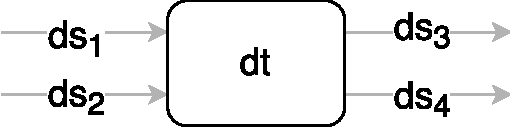
\includegraphics[width=0.35\textwidth]{img/example-data-transformation}
    \caption[Exemplo de transformação de dados]{Exemplo de transformação de dados, \( dt \), com dois conjuntos de dados de entrada, \( ds_1 \) e \( ds_2 \), e dois conjuntos de dados de saída, \( ds_3 \) e \( ds_4 \).}%
    \label{fig:example-transformation}
\end{figure}

No contexto de simulações computacionais, transformações de dados correspondem aos programas de simulação utilizados para executar um modelo computacional. 

\subsection{Conjunto de dados}

A especificação de um \textbf{conjunto de dados} \( ds \) é dada por \[ ds = (A, C) \] onde:
\begin{itemize}
    \item \( A = \{da_1, da_2, \ldots, da_{\delta} \} \) é um conjunto de atributos de dados; e
    \item \( C = \{dc_1, dc_2, \ldots, dc_{\zeta} \} \) é um conjunto de coleções de dados.
\end{itemize}

Em simulações computacionais, conjuntos de dados contêm os dados científicos comumente extraídos de arquivos produzidos pelos programas de simulação. Além disso, o termo coleção de dados é especificado formalmente na Subseção \ref{subsec:data-collection}.

\subsection{Atributo de dados}

Um \textbf{atributo de dados} é especificado da seguinte forma: \[ da = (\textrm{nome},\textrm{tipo}) \therefore \textrm{tipo} \in \{\textup{inteiro}, \textup{ponto flutuante}, \textup{texto}, \textup{arquivo}, \textup{booleano}\} \]

O nome do atributo de dados é um identificador que deve ser único em um mesmo conjunto de dados. O tipo do atributo provê um significado semântico ao mesmo. O exemplo da \autoref{tab:dataset-attributes-example} ilustra essa definição.

\begin{table}[htb]
    \centering
    \begin{tabular}{|c|c|}
        \hline
        \textbf{Nome do atributo} & \textbf{Tipo do atributo} \\
        \hline
        Nome             & texto           \\
        \hline
        Idade            & inteiro         \\
        \hline
        Altura \( (m) \) & ponto flutuante \\
        \hline
    \end{tabular}
    \caption[Exemplo de conjunto de dados com seus atributos de dados]{Exemplo de conjunto de dados de usuários com seus respectivos atributos.}%
    \label{tab:dataset-attributes-example}
\end{table}

\subsection{Coleção de dados}
\label{subsec:data-collection}

Uma \textbf{coleção de dados}, também chamada de conjunto de elementos de dados, é definida como \[ dc = \{ de_1, de_2, \ldots, de_{\eta} \} \] onde cada \( de \) é um elemento de dados.

\subsection{Elemento de dados}

Um \textbf{elemento de dados} é definido como

\[ de = \{ v_1, v_2, \ldots, v_{\theta} \} \therefore \#(ds.A) = \#(de) \]

onde o i-ésimo \( v \) é o valor do i-ésimo atributo de dados \( da \) de um conjunto de dados \( ds \). \( \#(ds.A) \) representa a cardinalidade do conjunto de atributos \( A \), \textit{i.e.}, a quantidade de atributos presentes no mesmo conjunto de dados \( ds \). Note que a quantidade de atributos do conjunto de dados \( ds \) deve ser igual à quantidade de valores presentes no elemento de dados \( de \).

Para exemplificar a relação entre coleção de dados e elemento de dados, considere a \autoref{tab:data-collections-and-data-elements}.

\begin{table}[htb]
    \centering
    \begin{tabular}{c|c|c|cc}
        & \textbf{Nome} & \textbf{Idade} & \textbf{Altura \((m)\)} \\
        \( de_{1} \) & Alice   & 22 & \( 1,77 \) & \rdelim\}{2}{.1mm}[\( dc_{1} \)] \\
        \( de_{2} \) & Bob     & 25 & \( 1,79 \) \\
        \( de_{3} \) & Charlie & 42 & \( 1,85 \) & \rdelim\}{1}{.1mm}[\( dc_{2} \)] \\
    \end{tabular}
    \caption[Relação entre coleção de dados e elemento de dados]{Relação entre coleção de dados e elemento de dados. Estes elementos de dados são instâncias do conjunto de dados de usuários da \autoref{tab:dataset-attributes-example}. Cada linha numerada da tabela é um elemento de dados; e existem duas coleções de dados: \( dc_{1} = \{de_{1}, de_{2}\} \) e \( dc_{2} = \{ de_{3} \} \).}%
    \label{tab:data-collections-and-data-elements}
\end{table}

\subsection{Dependência de dados}

Uma especificação de \textbf{dependência de dados} \( \phi \) é dada por \[ \phi = (ds, dt_{\textrm{previous}}, dt_{\textrm{next}}) \] onde:
\begin{itemize}
    \item \( ds \) é um conjunto de dados;
    \item \( dt_{\textup{previous}} \) é uma transformação de dados que {\bf produz} coleções de dados para o conjunto de dados \( ds \); e
    \item \( dt_{\textup{next}} \) é uma transformação de dados que {\bf consome} coleções de dados do conjunto de dados \( ds \).
\end{itemize}

\subsection{Um exemplo}%
\label{sec:um-exemplo-de-dataflow}

Para ilustrar as definições e especificações da \autoref{sec:dataflow}, vamos utilizar uma pequena amostra de um fluxo de dados real em dinâmica de fluidos computacionais. Na \autoref{fig:example-dataflow-specification} podemos ver o DAG correspondente a esse fluxo de dados \( D \): ele contém duas transformações de dados, \textsc{inputmesh} e \textsc{createequationsystems}, e três conjuntos de dados, \textsc{iinputmesh}, \textsc{oinputmesh} e \textsc{ocreateequationsystems}, assim como três dependências de dados. Eis a especificação de \( D \):

\begin{figure}[htb]
    \centering
    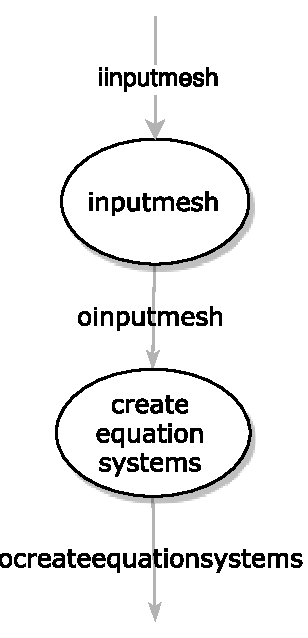
\includegraphics[width=0.35\textwidth]{img/example-dataflow-specification}
    \caption[Exemplo de especificação de fluxo de dados]{Exemplo de especificação de fluxo de dados, com duas transformações de dados e três conjuntos de dados.}%
    \label{fig:example-dataflow-specification}
\end{figure}

\[
    \begin{array}{rl}
    % \begin{cases}
        D = & (T, S, \Phi) \\
        S = & \{ \textsc{iinputmesh}, \textsc{oinputmesh}, \textsc{ocreateequationsystems} \} \\
        T = & \{ \textsc{inputmesh}, \textsc{outputmesh} \} \\
        \multirow{3}{*}{\Phi{} =}
            & \{ (\varnothing, \textsc{iinputmesh}, \textsc{inputmesh}), \\
            & (\textsc{inputmesh}, \textsc{oinputmesh}, \textsc{createequationsystems}), \\
            & (\textsc{createequationsystems}, \textsc{ocreateequationsystems}, \varnothing) \}
    \end{array}
    % \end{cases}
\]

\textbf{Observação:} o símbolo \( \varnothing \) denota \emph{nulo}, indicando que uma das transformações de dados correspondente à dependência de dados não existe.

Além disso, podemos ver alguns dos atributos de dados do conjunto de dados \textsc{iinputmesh} na \autoref{tab:iinputmesh-attributes}, assim como alguns de seus valores na \autoref{tab:iinputmesh-values}. Cada uma das linhas da \autoref{tab:iinputmesh-values} corresponde a um elemento de dados diferente, e todo o conjunto desses elementos de dados compõe toda a coleção de dados do conjunto de dados.

\begin{table}[htb]
    \centering
    \begin{tabular}{|c|c|}
        \hline
        \textbf{Nome do atributo} & \textbf{Tipo do atributo} \\
        \hline
        id & inteiro \\
        mesh{\_}file & arquivo \\
        dim & inteiro \\
        simulationid & inteiro \\
        restart{\_}control & booleano \\
        \hline
    \end{tabular}
    \caption[Atributos de dados do conjunto de dados \textsc{iinputmesh}]{Alguns dos atributos de dados do conjunto de dados \textsc{iinputmesh}.}%
    \label{tab:iinputmesh-attributes}
\end{table}

\begin{table}[htb]
    \centering
    \begin{tabular}{c|c|c|c|c}
        \textbf{id} & \textbf{mesh{\_}file} & \textbf{dim} & \textbf{simulationid} & \textbf{restart{\_}control} \\
        \hline
        1 & \texttt{/sedimentation/necker3d-1.msh} & 3 & 1 & \textrm{falso} \\
        2 & \texttt{/sedimentation/necker3d-2.msh} & 3 & 2 & \textrm{verdadeiro} \\
    \end{tabular}
    \caption[Valores dos atributos de dados de \textsc{iinputmesh}]{Alguns dos valores dos atributos de dados de \textsc{iinputmesh}.}%
    \label{tab:iinputmesh-values}
\end{table}

\section{Dados de proveniência}

\subsection{Definição}

% upstream: http://www.aulete.com.br/proveni%C3%AAncia
O dicionário Aulete Digital~\cite{aulete2014dicionario} define \textbf{proveniência} como
``lugar de onde alguém ou alguma coisa provém; origem; fonte''. Em simulações computacionais, a proveniência nos ajuda a interpretar e entender resultados. Através da examinação e da cadeia de passos que criaram um certo resultado, nós podemos: (\(i\)) verificar que o experimento foi realizado de acordo com os procedimentos aceitáveis; (\(ii\)) inspecionar as suas entradas; e, em alguns casos, (\(iii\)) reproduzir os mesmos resultados~\cite{freire2008provenance}.

Questões básicas sobre dados científicos podem ser respondidas por meio do conhecimento e da introspecção de sua proveniência, tais como

\begin{enumerate}
    \item quem criou o dado, e quando foi essa criação?
    \item quem modificou o dado, e quando essa modificação ocorreu?
    \item que processo criou o dado?
    \item que outros dados foram produzidos a partir dos dados originais?
\end{enumerate}

Um dos componentes mais importantes que podemos obter com proveniência são suas informações sobre \textbf{causalidade}, isto é, a relação de dados de entrada que, associados a um processo, levam a um determinado conjunto de dados de saída~\cite{freire2008provenance}. A causalidade pode ser representada através de fluxos de dados e de grafos --- onde os nós correspondem a processos e arestas correspondem a dados científicos ---, como no exemplo da \autoref{sec:um-exemplo-de-dataflow}.

Um segundo exemplo relevante de componente de proveniência são as informações definidas e providas pelo usuário, as quais não podem ser capturadas automaticamente~\cite{freire2008provenance}. Esse tipo de informação é usualmente provido em níveis de granularidade arbitrários através de anotações e observações do usuário.

\subsection{Categorias de dados de proveniência}%
\label{subsec:categorias-de-dados-de-proveniencia}

Existem dois tipos de dados de proveniência envolvidos na gerência de fluxo de dados: \textbf{prospectiva} e \textbf{retrospectiva}~\cite{murta2014noworkflow,freire2008provenance}:

\begin{itemize}
% murta2014noworkflow ++ freire2008provenance
    \item A \textbf{proveniência prospectiva} contempla a especificação e a estrutura de uma tarefa computacional --- por exemplo, um \textit{script}, ou um programa de simulação --- e associa a ela os passos que precisam ser seguidos para gerar um conjunto de dados. Ela corresponde à definição de um fluxo de dados e ao seu grafo, transformações de dados e dados científicos relacionados. Assim, a proveniência prospectiva é uma descrição do próprio processo computacional~\cite{mcphillips2015yesworkflow}.
% murta2014noworkflow ++ freire2008provenance
    \item Por outro lado, a \textbf{proveniência retrospectiva} captura não apenas os passos executados de uma tarefa computacional, mas também informações relacionadas ao ambiente e tempo de execução da mesma - por exemplo, quais parâmetros foram passados aos programas, qual \abbrev{PID}{Process ID} processo (PID) do sistema operacional foi executado, por quem o PID foi executado, qual foi a duração total (incluindo seus instantes de início e de fim) do mesmo, ou quais variáveis de ambiente do sistema operacional estavam definidas. Sua estrutura do grafos respeita à especificação provida pela proveniência prospectiva.
\end{itemize}

Por meio dos dois tipos citados de dados de proveniência, um sistema de fluxo de dados é capaz de orquestrar e prover diferentes níveis de abstração para a execução de uma simulação científica~\cite{murta2014noworkflow}, os quais são inexistentes em programas de simulação, tais como \textit{scripts}. Como iniciativas para a gerência de dados de proveniência, pode-se citar o NoWorkflow~\cite{murta2014noworkflow}, o YesWorkflow~\cite{mcphillips2015yesworkflow}, o DfAnalyzer~\cite{silva2016situ} e a biblioteca Tigres~\cite{hendrix2016tigres}.

Ademais, a captura de dados de proveniência pode ser realizada de duas formas distintas, \textit{offline} e \textit{online}~\cite{silva2015propostadoutorado}. A captura \textit{offline} consiste em armazenar os dados de uma simulação computacional em um determinado repositório logo \textbf{após} a execução da mesma --- por exemplo, como realizado pelo Kepler~\cite{ludascher2006scientific}. Em contrapartida, a captura \textit{online} consiste na obtenção e no armazenamento de dados \textbf{em tempo de execução}, como realizado no Pegasus~\cite{deelman2005pegasus} e no Swift/T~\cite{zhao2007swift}.

Uma simples observação é que o desempenho da captura de proveniência \textit{online} tende a ser ligeiramente pior do que a \textit{offline}, devido à possível sobrecarga do armazenamento de dados de proveniência concorrentemente ao processamento dos programas de simulação. Em outra perspectiva, vale enfatizar que a captura \textit{online} é mais flexível e tem um potencial analítico maior, pois permite que os usuários realizem consultas mesmo antes do término da simulação, o que possui um valor inestimável, uma vez que simulações computacionais são comumente realizadas em larga escala e, portanto, custosas e demoradas.

\subsubsection{Exemplo com dados de proveniência}

Para ilustrar a diferença entre os dois tipos de dados de proveniência apresentados, considere o clássico exemplo de contagem de palavras\footnote{Cujo objetivo é obter a ordem decrescente de frequência das palavras que aparecem no texto.} (\textit{word count}), no qual o conjunto de dados inicial é um arquivo de texto em \abbrev{ASCII}{American Standard Code for Information Interchange} ASCII. A primeira tarefa de processamento é a leitura e subsequente análise do arquivo de texto a fim de extrair palavras do mesmo. A segunda etapa é realizar a contagem das palavras a partir da lista de palavras obtida no passo anterior. Finalmente, o último passo de processamento é ordenar em ordem descrescente a frequência de palavras obtidas no passo anterior.

A proveniência prospectiva desse experimento poderia ser representada através do grafo da \autoref{fig:word-count-prospective}. Por outro lado, a proveniência retrospectiva do último passo (ordenação) poderia ter capturado em tempo de execução algumas das informações presentes na \autoref{tab:word-count-retrospective}. Sendo assim, dependendo das análises desejadas pelos usuários de domínio, a proveniência prospectiva não é suficiente. Além disso, no contexto da análise exploratória de arquivos de dados científicos, os usuários estão comumente interessados em dados de proveniência retrospectiva. Mais especificamente, eles necessitam investigar dados de domínio presentes nos arquivos produzidos pelos programas de simulação.

\begin{figure}[htb]
    \centering
    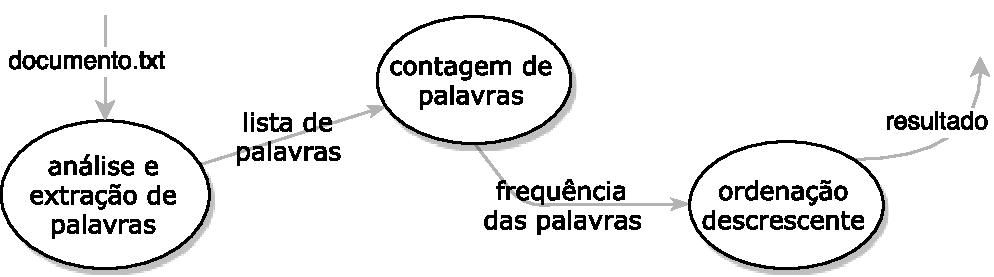
\includegraphics[width=\textwidth]{img/word-count-prospective}
    \caption[Proveniência prospectiva do exemplo de contagem de palavras]{Proveniência prospectiva do exemplo de contagem de palavras.}%
    \label{fig:word-count-prospective}
\end{figure}

\begin{table}[htb]
    \centering
    \begin{tabular}{r|l}
        \hline
        \textit{Timestamp} de início & 2017-06-25 03:11:05.231                         \\
        \textit{Timestamp} de fim    & 2017-06-25 03:11:09.586                         \\
        PID                          & 4671                                            \\
        Linha de comando             & \texttt{./sort --order=desc --in=freq-list.csv} \\
        Variáveis de ambiente        & \texttt{PWD=/home/tperrotta;PATH=/usr/bin:/bin} \\
        Usuário                      & tperrotta                                       \\
        \hline
    \end{tabular}
    \caption[Proveniência retrospectiva do exemplo de contagem de palavras]{Proveniência retrospectiva do exemplo de contagem de palavras da etapa de ordenação decrescente.}%
    \label{tab:word-count-retrospective}
\end{table}

\section{Rastreamento de dados de proveniência}%
\label{sec:rastreamento-de-dados-de-proveniencia}

As soluções precisam ser capazes de \textbf{rastrear} e \textbf{monitorar} o fluxo de dados que são consumidos e produzidos por cada transformação de dados (programa de simulação) durante a sua execução. Nesse contexto, dois níveis de abstração existem para tratar a \textbf{gerência do fluxo de dados}: o físico e o lógico~\cite{silva2015propostadoutorado}.

\subsection{Gerência do fluxo de dados no nível físico}%
\label{sec:gerencia-do-fluxo-de-dados-no-nivel-fisico}

A \textbf{gerência do fluxo de dados no nível físico}, ou \textbf{rastreamento físico de dados de proveniência}, consiste no apoio às \emph{transformações de dados} no nível do sistema de arquivos, \textit{i.e.}, rastreando \emph{o fluxo de arquivos}. Nessa abordagem, é necessário etiquetar cada arquivo com um identificador único, como uma URL (\textit{Uniform Resource Locator}), dentro do mesmo conjunto de dados~\cite{silva2015propostadoutorado}. Esse tipo de proveniência captura muitos detalhes, os quais podem ser úteis na depuração de simulações computacionais devido à sua gerência dos arquivos consumidos e produzidos por cada transformação de dados~\cite{silva2017raw}.

Nesse contexto, as transformações de dados são analisadas apenas no que tange o consumo e a produção de arquivos (e elementos de dados) por cada programa científico, sem considerar dados de domínio da simulação. Assim, essas transformações de dados são análogas a caixas-pretas (do inglês, \textit{black box})~\cite{silva2017raw}, já não proveem índices ou qualquer tipo de suporte à consulta em termos do conteúdo de domínio da simulação. Desse modo, os usuários limitam-se apenas a ponteiros para os elementos de dados nos arquivos envolvidos no fluxo de dados, requerendo-se que os mesmos façam análises individuais de cada arquivo para poder extrair algum significado semântico deles~\cite{silva2015propostadoutorado}.

\subsection{Gerência do fluxo de dados no nível lógico}%
\label{sec:gerencia-do-fluxo-de-dados-no-nivel-logico}

Em contrapartida, a \textbf{gerência do fluxo de dados no nível lógico}, ou \textbf{rastreamento lógico de dados de proveniência}, consiste no monitoramento de \emph{como} os elementos de dados são consumidos e produzidos pelas transformações de dados e programas científicos. Tais elementos de dados apresentam o conteúdo de arquivos de dados científicos e, a partir da sua gerência, os seus relacionamentos podem ser utilizados para a \emph{reconstrução do fluxo de dados}. Dessa maneira, menos dados precisam ser armazenados, já que um fluxo de dados costuma ter bem menos transformações de dados do que elementos de dados~\cite{silva2015propostadoutorado} (nível de granularidade grosso).

No que diz respeito aos usuários, consultas podem ser realizadas de forma direcionada aos aspectos do domínio da simulação computacional, sem a necessidade de se fazer uma etapa de análise prévia (diferentemente da gerência no nível físico). Além disso, o rastreamento lógico de dados pode ser \emph{automaticamente} derivado das especificações das transformações de dados, uma vez que elas já apresentam propriedades sobre conjuntos de dados consumidos e produzidos~\cite{ikeda2013logical,silva2017raw}. Por outro lado, vale destacar que o custo computacional é maior para a gerência de dados no nível lógico do que no físico, uma vez que nesse tipo de gerência os elementos de dados precisam ser capturados e monitorados em tempo de execução, enquanto que no nível físico esse monitoramento resume-se à utilização de ponteiros de arquivos para os dados científicos, antes mesmo da execução.

% \subsection{Um exemplo}

% Para ilustrar a diferença entre os conceitos apresentados na \autoref{sec:gerencia-do-fluxo-de-dados-no-nivel-fisico} e na \autoref{sec:gerencia-do-fluxo-de-dados-no-nivel-logico}, \perrotta{REVIEW: Dar um exemplo que ilustre a diferença entre gerência de dados nos níveis físico e lógico. Eu me lembro da parte física (taskid), mas estou confuso na parte lógica, então vou delegar isso para mais tarde.}

% \missingfigure{REVIEW: Exemplo para ilustrar: diferença entre físico e lógico}

% \begin{lstlisting}[language=SQL,caption={},label=]
% SELECT * FROM table WHERE task_id = task_id;
% \end{lstlisting}

\subsection{Mapeamento de atributos}%
\label{subsec:mapeamento-de-atributos}

A seguinte definição foi extraída, traduzida e adaptada de~\cite{ikeda2013logical}:

\textbf{Definição(mapeamento de atributo)}: seja \( dt \) uma transformação de dados com um conjunto de dados de entrada \( I \) e um conjunto de dados de saída \( O \). Assume-se também que \( A \) é um atributo de \( I \) e \( B \) é um atributo de \( O \). Diz-se que \( dt \) tem um mapeamento de atributo entre o atributo de entrada \( I.A \) e o atributo de saída \( O.B \), denotado por \( I.A \leftrightarrow O.B \), se todos os possíveis valores de \( x \in \textrm{domínio}(B) \) e todas as possíveis instâncias do conjunto de entrada \( I^{\prime} \) satisfazem
\[ \sigma_{B=x}(T(I^{\prime})) = \sigma_{B=x}(T(\sigma_{A=x}(I^{\prime}))) \]

Em outras palavras, e de forma simplificada, existe um mapeamento de atributos entre \( A \) e \( B \) quando:

\begin{enumerate}
    \item \( A \) faz parte de um conjunto de dados de entrada de uma transformação \( dt \), e \( B \) faz parte de um conjunto de dados de saída de \( dt \), ou vice-versa;
    \item \( A \) e \( B \) possuem o mesmo tipo; e
    \item \( A \) e \( B \) possuem o mesmo nome.
\end{enumerate}

Por exemplo, considere que temos um conjunto de dados \( ds_{1} \) com dois atributos \( x \) e \( y \) do tipo ponto flutuante, representando as coordenadas de um plano, e uma transformação \( dt \) que dobra os valores de cada uma dessas coordenadas e é aplicada a \( ds_{1} \), produzindo \( ds_{2} \). Nesse cenário, existem dois mapeamentos de atributos: \( ds_{1}.x \leftrightarrow ds_{2}.x \) e \( ds_{1}.y \leftrightarrow ds_{2}.y \).
